\documentclass{beamer}
\mode<presentation>
% \usetheme{default}
% \usetheme{Boadilla}
% \usetheme{Madrid}
% \usetheme{Montpellier}
 \usetheme{Warsaw}
% \usetheme{Copenhagen}
% \usetheme{Goettingen}
% \usetheme{Hannover}
% \usetheme{Berkeley}
 
% \usecolortheme{crane}
 % \beamertemplatesolidbackgroundcolor{craneorange!25}
 
 \usepackage[utf8]{inputenc}
%\usepackage[T1]{fontenc}
\usepackage{amsmath,amssymb}
\usepackage[english,french]{babel}
\usepackage{multimedia}

%\usepackage{natbib}


 
\header{
\includegraphics[height=1.5cm]{phelma.jpg} \hfill 
\includegraphics[height=1.6cm]{cea2.png} \hfill 
\includegraphics[height=1.6cm]{ujf.jpg}}
 

\title[Translocation de biomolécules à travers un nanopore]{Etude théorique de la translocation de biomolécules à travers un nanopore}




 
\author{Timothée Menais}
 
\institute[CEA] {
\includegraphics[height=1.4cm]{spram.jpg} \hspace{0.3cm}

\includegraphics[height=1.2cm]{inac.jpg}}


\setbeamertemplate{navigation symbols}{}


\begin{document}
\selectlanguage{french}

\frame[plain]{\titlepage} % # 1

\frame % 1
{
  \frametitle{Introduction}
 
 
 \begin{itemize}
 
 \begin{center}
 \item<1-> Translocation d'ADN à travers un nanopore
 
 \medskip
 \item<2-> Intérêts technologiques et fondamentaux
 
 \medskip
 \item<3> Arrivée du graphène
 \end{center}
 
 \end{itemize}


}




\frame{\tableofcontents}


\section{Systèmes étudiés}
 
 \frame % # 2
{
  \frametitle{Nature de l'ADN}
  
  \begin{columns}
  \begin{column}{0.7\textwidth}
\begin{center}
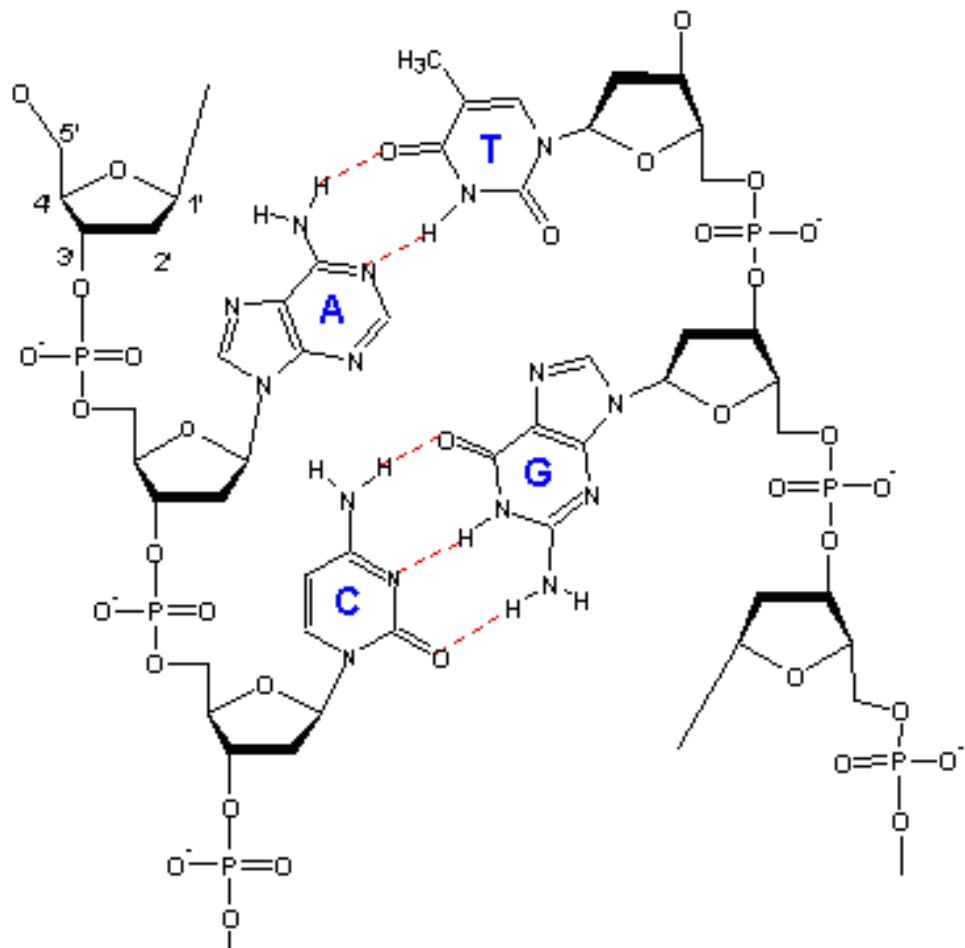
\includegraphics[width=0.8\textwidth]{adn.jpg}
\end{center}
\end{column}

  \begin{column}{0.3\textwidth}
\begin{center}
Structure\\
\medskip

Liaisons covalentes\\
\medskip

Liaisons hydrogènes\\
\medskip
Interactions orbitalaires


\end{center}
\end{column}

\end{columns}

}


\frame % 3
{
  \frametitle{Translocation}
 

\begin{columns}
 \begin{column}{0.8\textwidth}
\begin{center}
  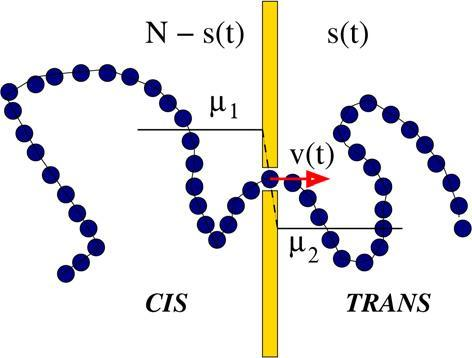
\includegraphics[width=0.8\textwidth]{translocation.jpg} 
 \end{center}
\end{column}
\begin{column}{0.3\textwidth}

 \begin{center}
\begin{itemize}
\item<2->{ $\tau = N^\alpha f^{-\delta}$}
\medskip

\item<3->{ exposants critiques}
\end{itemize}


\end{center}
 
\end{column}
\end{columns}
}

\frame
{
\frametitle{Pores classiques}

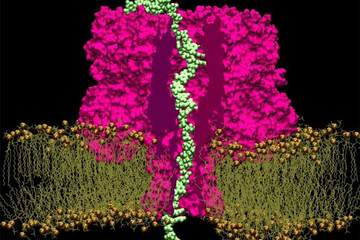
\includegraphics[width=0.54\textwidth]{biopore.jpg}\hspace{0.02\textwidth} 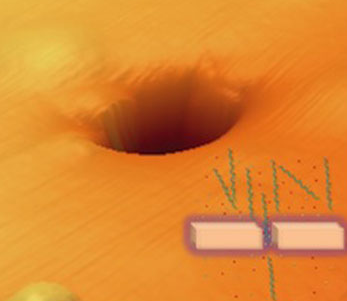
\includegraphics[width=0.42\textwidth]{artificialpore.png}
\medskip
\begin{center}
\uncover<2->{Problèmes d'épaisseur}
\end{center}

}


\frame
{\begin{center}


\frametitle{Nanopores dans le graphène}
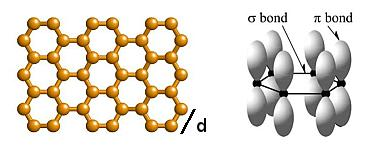
\includegraphics[width=0.7\textwidth]{orbitals2.jpg} 

\uncover<2->{cristal bidimensionnel de carbones aromatiques}

\uncover<3->{ 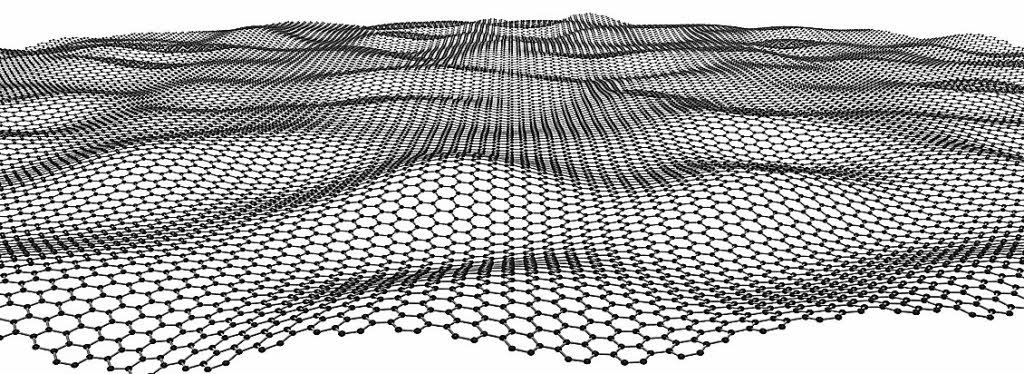
\includegraphics[width=0.7\textwidth]{vib.jpg}
}

\end{center}
}

\section{Modèle numérique}

 
\frame % # 2
{
  \frametitle{Exemple}
\begin{center}
Exemple de modèle gros grain
\end{center}  
  
 \begin{columns}
 \begin{column}{0.6\textwidth}

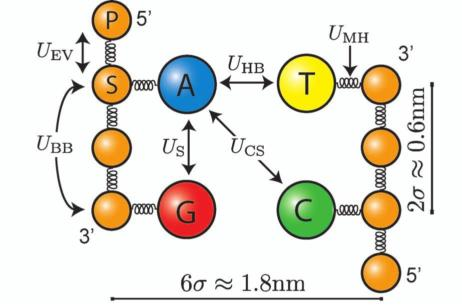
\includegraphics[width=\textwidth]{moldyn2.jpg}
\end{column}
\begin{column}{0.4\textwidth}



\begin{itemize}

\item<2-> Interactions de contact 
\medskip


 \item<3-> Liaisons covalentes
 \medskip

 
 \item<4-> Potentiel de tortion
 \medskip
 
 \item<5-> Interactions hydrogènes
 \medskip
 
 \item<6-> Interactions orbitalaires
\end{itemize}




 
\end{column}

\end{columns}
\medskip

\uncover<7->{ \centering Dynamique moléculaire: $\frac{d \textbf{r}_n}{dt} = -\frac{1}{\epsilon}\frac{\partial F_{tot}}{\partial \textbf{r}_n} +\textbf{g}_n$} 

\vfill
{\tiny

\usebibitemtemplate{\color{structure}\insertbiblabel} 
\usebibliographyblocktemplate{\color{structure}}{\color{black}}{\color{structure!75}}{\color{structure!75}} 

\begin{thebibliography}{} 
\bibitem[référence]{jchem}
M. C. Linak, R. Tourdot, and K. D. Dorfman. 
\newblock {Moving beyond watson–crick models of coarse grained
dna dynamics
}. 
\newblock The Journal of Chemical Physics, vol. 135, no. 20, p. 205102, 2011.
 

\end{thebibliography} }
}


\frame % # 2
{
  \frametitle{Notre modèle}
 
\begin{center}

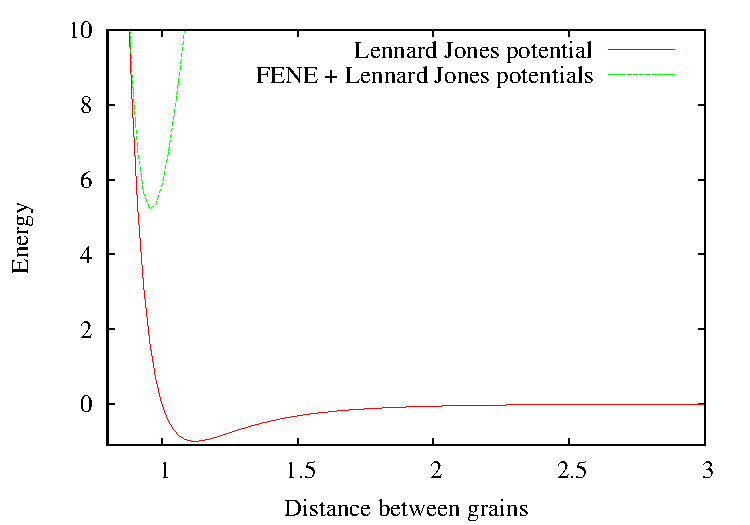
\includegraphics[width=0.72\textwidth]{potentials.pdf}


\begin{itemize}
\begin{center}
\item<2-> Interactions de contact, coeur dur et VdW
\medskip


 \item<3-> Liaisons covalentes, ajout de $\ln\left[1-(r/r_o)^2\right]$
 \medskip

 \end{center}
\end{itemize}
\end{center}
}

\frame % # 2
{
  \frametitle{Notre modèle}
 
\begin{center}

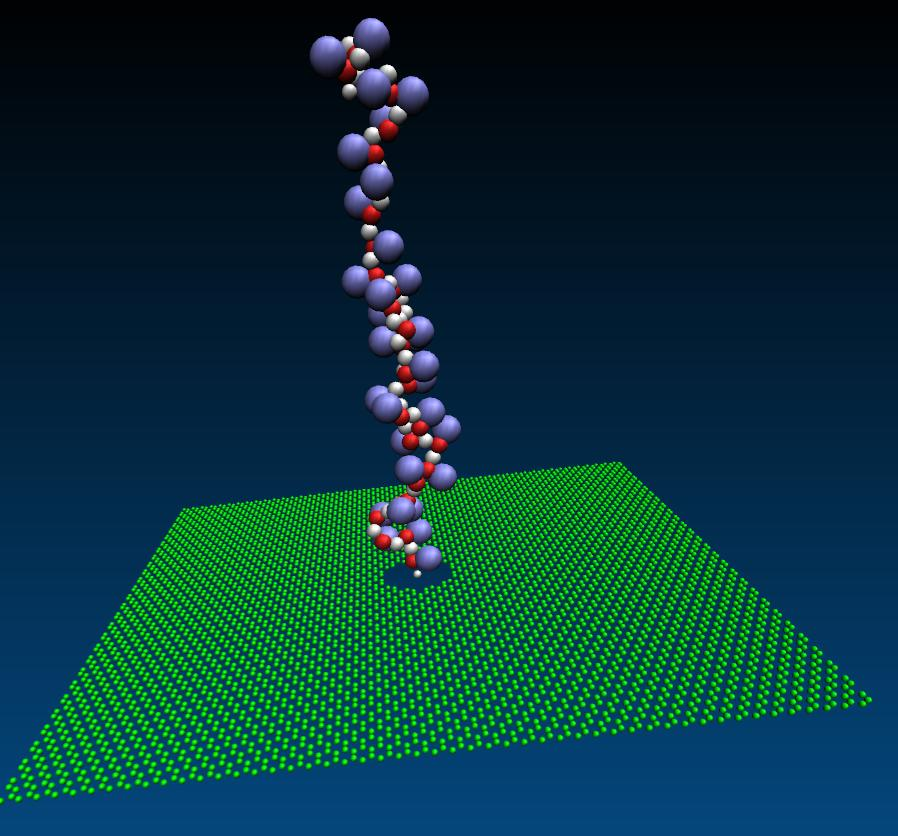
\includegraphics[width=0.6\textwidth]{systemmodlo.jpg}

4ème grain, carbones, interactions $\pi$/$\sigma$

\end{center}
}

\section{Théorie et résultats}

\frame % # 2
{
  \frametitle{Statique}
 \centering
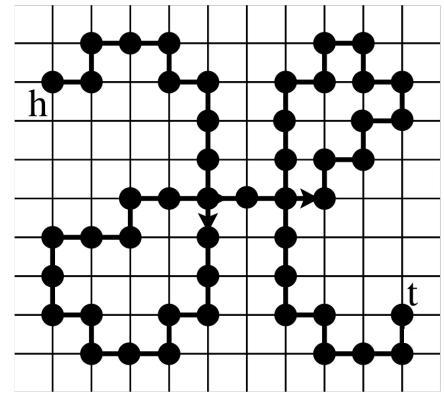
\includegraphics[width=0.5\textwidth]{resideal.jpg}
\medskip

$\left<\textbf{r}\right> =0$ et $\left<\textbf{r}^2\right> =b^2 N$

}

\frame % # 2
{
  \frametitle{Statique}

\begin{columns}
 \begin{column}{0.55\textwidth}

\begin{itemize}

 \item<1-> Cas idéal
 \medskip

 
 \item<2->$R_0\propto b N^{\frac{1}{2}} $
 \medskip
 
 \item<3->$P(\textbf{r},N)=\left(\frac{3}{2\pi N b^2}\right)^\frac{3}{2}\exp\left(-\frac{3\textbf{r}^2}{2 N b^2}\right)$
 \medskip
 \item<4->$F(\textbf{r})= F(0)+\frac{3k_BT\textbf{r}^2}{2Nb^2}$


\end{itemize}
 
\end{column}
 
\begin{column}{0.55\textwidth}

\begin{itemize}


\item<1-> Marche auto-évitante
\medskip

 
 \item<2->$R_0\propto b N^\nu $( $\nu \approx 3/5$, exp. de Flory)
 \medskip
 
 \item<3->$P_{SAW}(R,N) \propto \exp\left[-\frac{3\textbf{r}^2}{2 N b^2}-\frac{v_cN^2}{2\textbf{r}^3}\right]$
 \medskip
 
 \item<4->$F(\textbf{r})= F(0)+\frac{3k_BT\textbf{r}^2}{2Nb^2}+\frac{k_BTv_cN^2}{2\textbf{r}^3}$


\end{itemize}
 
\end{column}
\end{columns}
}

\frame % # 2
{
  \frametitle{Dynamique de Rouse}
\centering
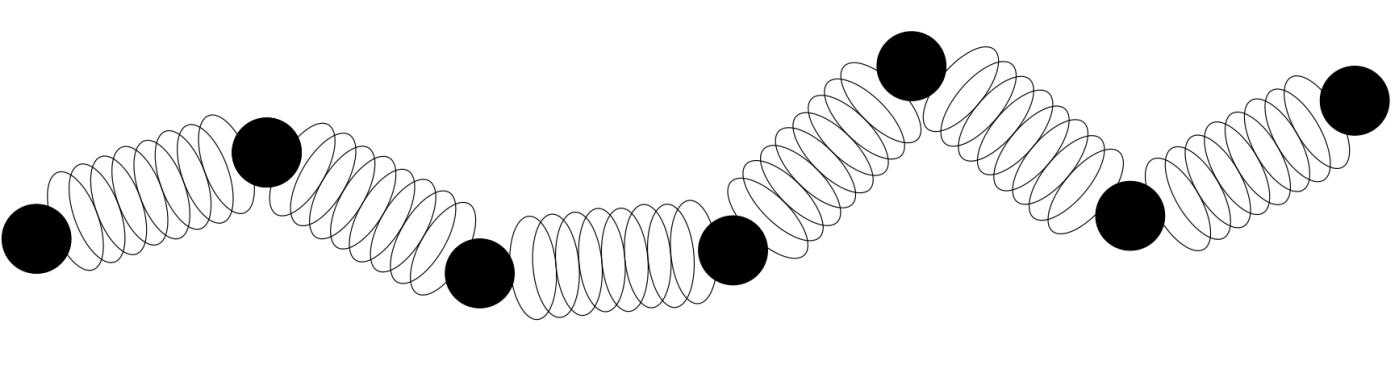
\includegraphics[width=0.8\textwidth]{rouse.jpg}






\begin{itemize}


\item<2-> \begin{center} $\left<(\textbf{r}_{CM}(t)-\textbf{r}_{CM}(0))^2\right> =\frac{6 k_B T}{N \epsilon} t = 6 D t$
\medskip

\item<3-> traction: $v\propto \eta F \propto N\epsilon F$

\medskip

\item<4-> vérifications indépendantes

\end{center}
\end{itemize}

}



\frame
{\frametitle{Statique}
\centering
 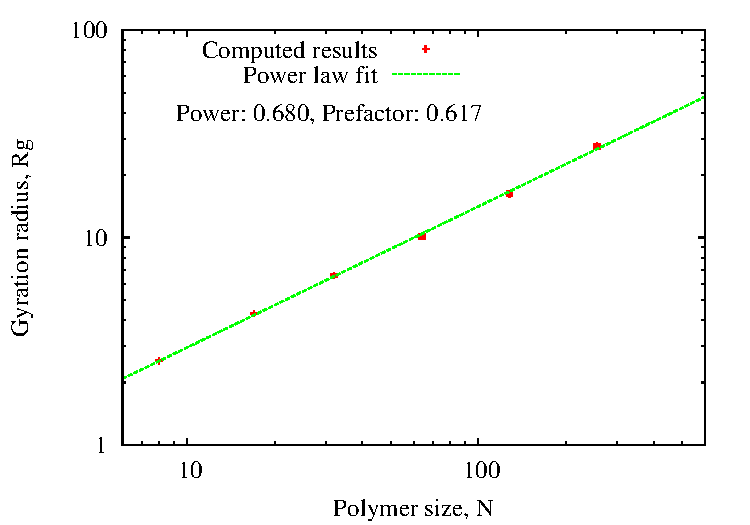
\includegraphics[width=0.9\textwidth]{gyrationradius.pdf}
}


 

\frame
{\frametitle{Théorème de fluctuation-dissipation}



{\centering
\makebox[0pt]{%
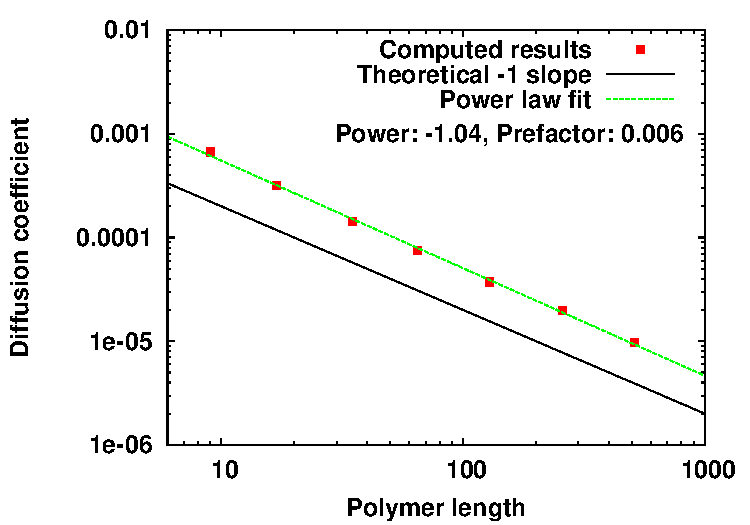
\includegraphics[width=0.6\textwidth]{diffusioncoefficient.pdf}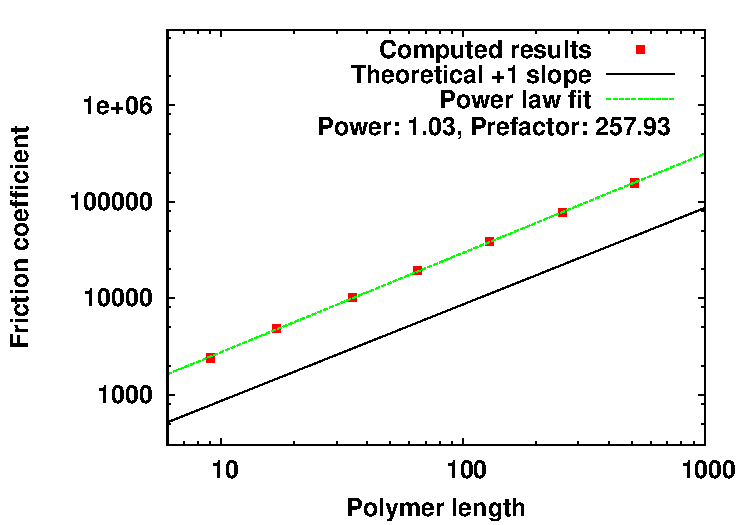
\includegraphics[width=0.6\textwidth]{penteforce.pdf}
}\par
}
\begin{center}
Resultats conformes à la théorie, théorème de fluctuation-dissipation vérifié.
\end{center}

}

\frame
{\frametitle{Polymère greffé}
\begin{center}
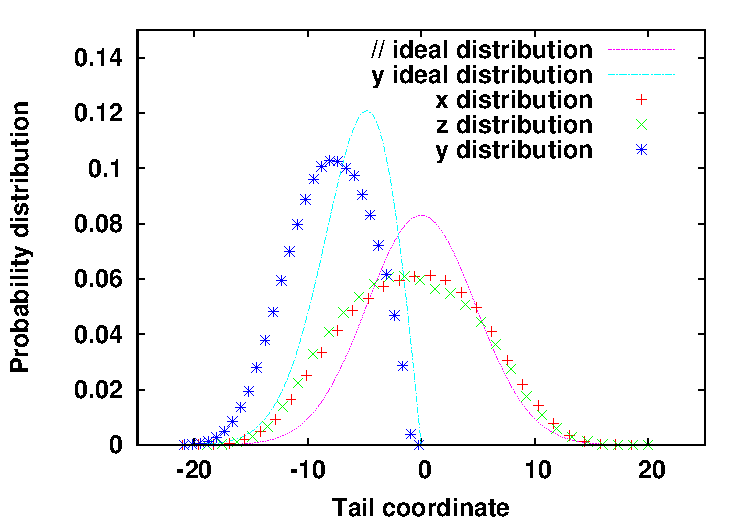
\includegraphics[width=0.9\textwidth]{probdistribution.pdf}

\end{center}

}



\frame % 3
{
  \frametitle{Translocation}
  

  \begin{center}
   \uncover<1->{ cas non biaisé: $\tau$ est proportionnel à $\frac{R_0^2}{D}$ $_\tilde{}$ $N^{1+2\nu}$}
   \medskip
   
   \uncover<2->{ biaisé:$\tau \propto N^{2\nu}$ à $\tau \propto N^{1+\nu}$}
   \medskip
   
    \uncover<3->{ $\tau \propto F^{-1}$ à $\tau \propto F^{(1/\nu)-2}$}
  \end{center}

}

}


\frame
{\frametitle{Pore large}

{\centering
\makebox[0pt]{%
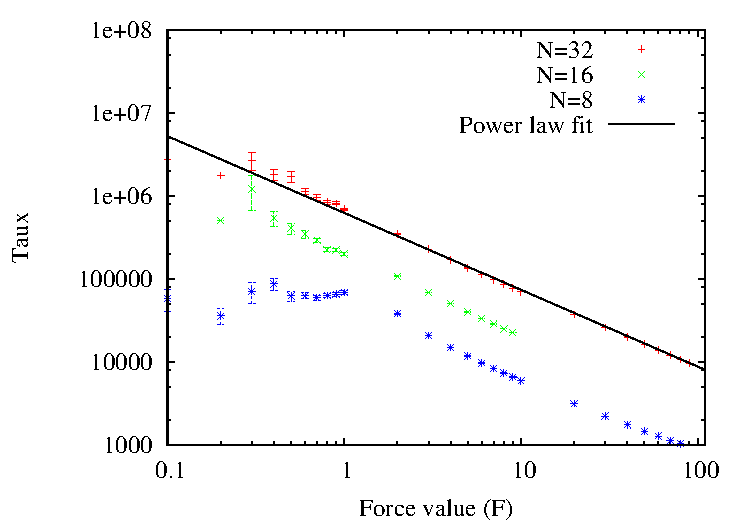
\includegraphics[width=0.6\textwidth]{translocfholebigger.pdf} 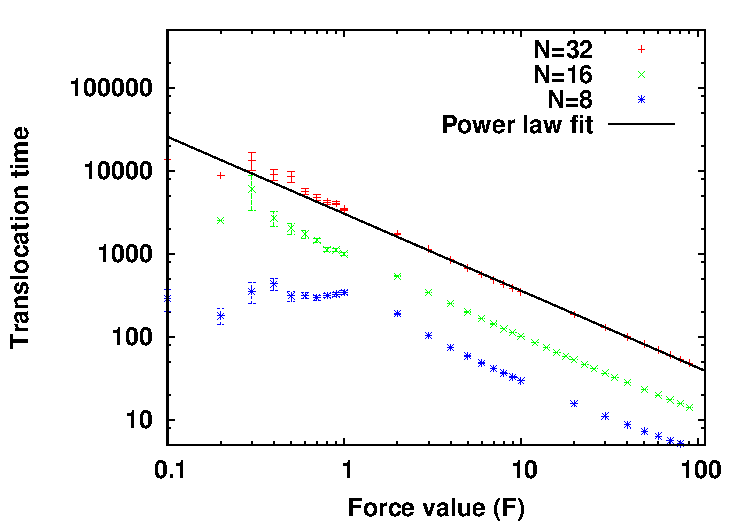
\includegraphics[width=0.6\textwidth]{translocholebigger.pdf}
}\par
}
\begin{center}
\uncover<2->{Deux régimes, $\tau\propto 1/F$ et exposant critique plus élevé}
\medskip

\uncover<3->{$\tau\propto N^{1.69} \approx N^{1+\nu}$}
\end{center}

}

\frame
{\frametitle{Pore étroit}

{\centering
\makebox[0pt]{%
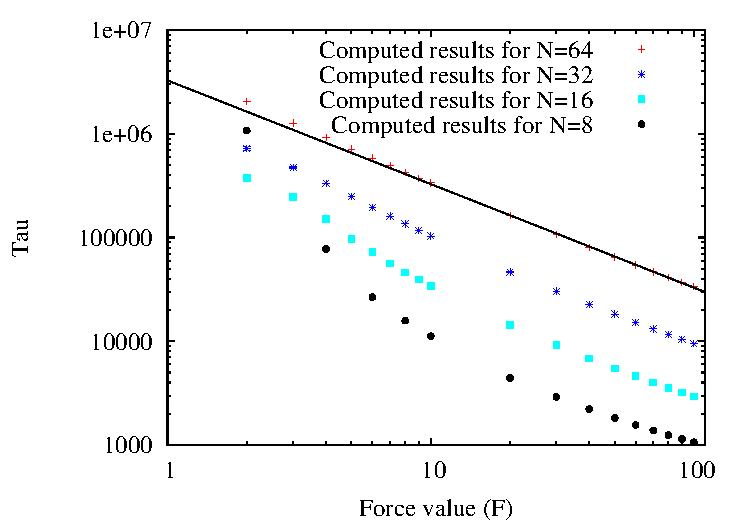
\includegraphics[width=0.6\textwidth]{translocfthinpore.pdf} 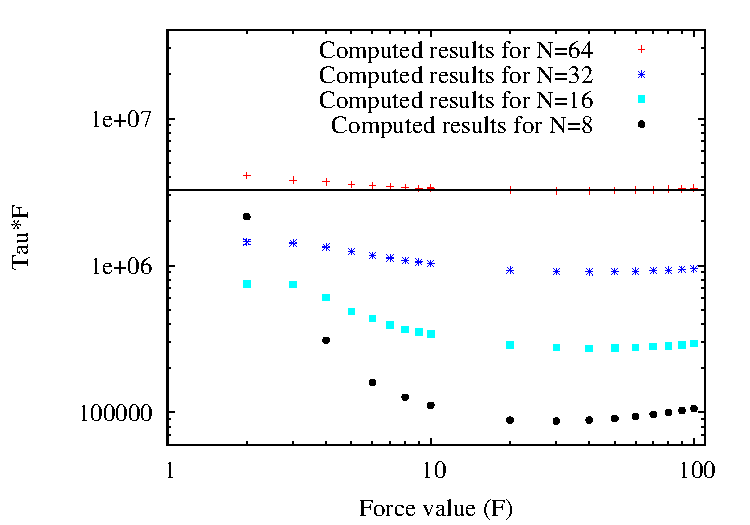
\includegraphics[width=0.6\textwidth]{translocthinpore.pdf}
}\par
}

\begin{center}
\uncover<2->{Toujours deux régimes pour les forces}
\medskip

\uncover<3->{$\tau\propto N^{1+\nu}$}
\end{center}
}

\frame
{\frametitle{Comparaison}

{\centering
\makebox[0pt]{%
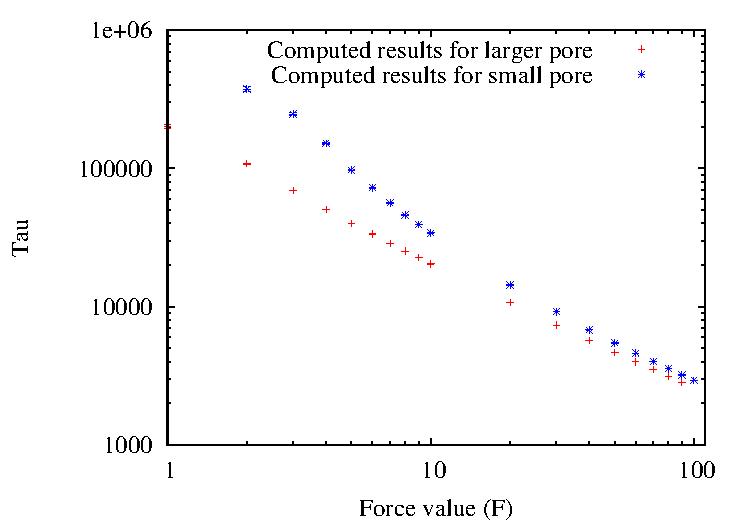
\includegraphics[width=0.6\textwidth]{translocporedifn.pdf} 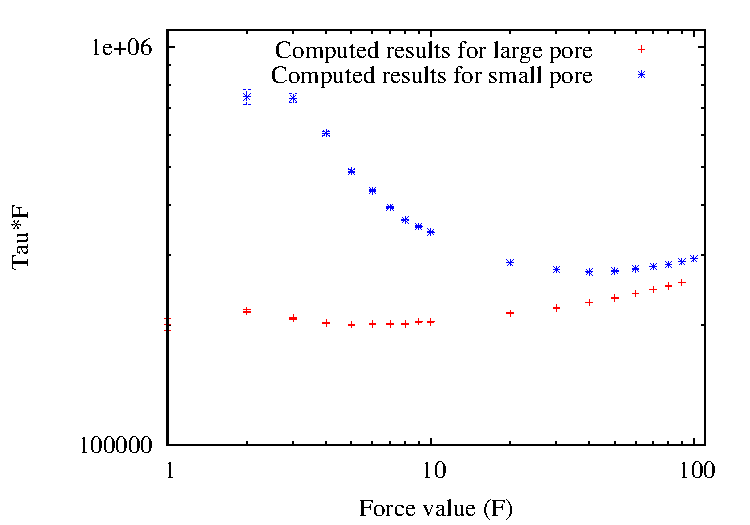
\includegraphics[width=0.6\textwidth]{translocporedif.pdf}
}\par
}
\begin{center}
Ralentissement de la translocation avec un pore étroit
\end{center}

}

\frame
{\frametitle{Pore vibrant}

{\centering
\makebox[0pt]{%
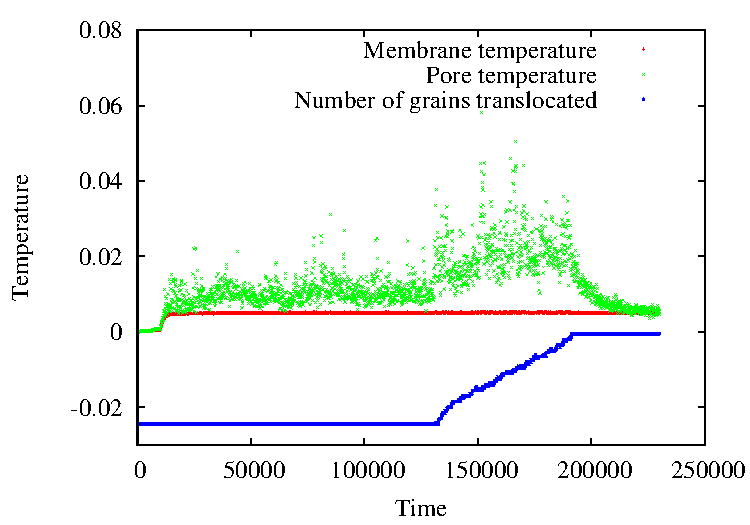
\includegraphics[width=0.6\textwidth]{tempmurmobil.pdf}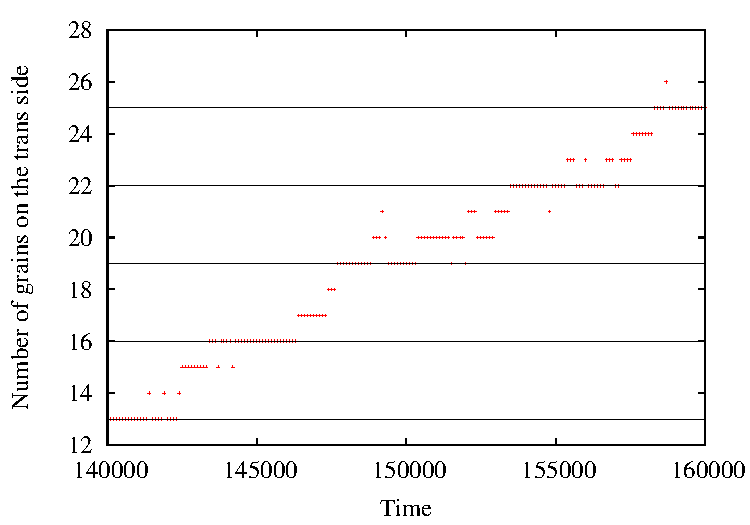
\includegraphics[width=0.6\textwidth]{murmobil.pdf}
}\par
}
\begin{center}
Echauffement du pore et translocation fractionnée
\end{center}

}








%\section*{Conclusion}

\frame % 3
{
  \frametitle{Conclusion}
 
 
 \begin{itemize}
 
 \begin{center}
 \item Utilisation d'un modèle original
 \pause
 \medskip
 \item Détermination de lois d'échelle
 \pause
 \medskip
 \item Effets du frottements du pore
 \pause
 \medskip
 \item Cas du pore vibrant?
 \pause
 \medskip
 \item Flexibilité de l'ensemble du plan?
 \end{center}
 
 \end{itemize}


}

\frame % 3
{
  \frametitle{Conclusion}
 
 
 
 
 \begin{center}
 {\HUGE Merci de votre attention.
 
 
 \pause
 \medskip
 Des questions ?}
 \end{center}
 
 


}





\end{document}
       
 